% !TEX root = ../main.tex

\clearpage
\appendix



\section{Training and Data Processing Details}
\label{app:implementation}

\subsection{Trajectory-Quality Annotations}
\label{app:quality_annotations}

We use two numerical quality scales according to annotation granularity.
\emph{Episode-level annotation} uses a 1--12 scale, with rollout scores in $[1,10]$ and expert demonstrations assigned $q^\star=12$.
\emph{Coarse-level annotation} uses a 1--5 scale, with rollout scores in $\{1,2,3,4\}$ and expert demonstrations assigned $q^\star=5$.
In all settings, every failed trajectory receives $q=1$.
Expert demonstrations are treated as optimal reference trajectories and assigned scores above the rollout range; the same expert score is used at deployment.
Each score is assigned to a complete trajectory and inherited by all training segments extracted from it.

\textbf{RoboChallenge Table30-V2.}
We use human episode-level annotations from the official RoboChallenge platform.
Platform operators already rate each rollout on a 1--10 scale according to task completion, with successful trajectories typically receiving scores of at least 8.5.
We directly use these platform ratings as rollout quality scores, except that all failed trajectories are assigned $q=1$.
Expert demonstrations receive $q^\star=12$.

\textbf{Single-task shirt-folding post-training.}
We likewise use human episode-level annotation.
After each rollout, the data collector assesses task completion before resetting the scene and assigns a score on a 1--10 scale, following the same completion-based scoring approach as RoboChallenge.
Failed trajectories receive $q=1$, and task-specific expert demonstrations receive $q^\star=12$.

\textbf{RoboTwin~2.0.}
We apply coarse-level annotation separately to rollouts from expert-trained LoopWAM, X-VLA, and $\pi_{0.5}$.
For each policy, we compute its overall rollout success rate across all tasks and manually inspect approximately 0.7\% of its trajectories for motion smoothness and action accuracy.
These two assessments determine a single shared score for all successful trajectories from that policy across tasks; every failed trajectory receives $q=1$.
Expert-trained LoopWAM achieves approximately 90\% success during rollout collection and produces relatively smooth trajectories, so its successful rollouts receive $q=4$.
X-VLA and $\pi_{0.5}$ each achieve less than 50\% success and produce less smooth trajectories, so their successful rollouts receive $q=3$.
Expert demonstrations receive $q^\star=5$.

\textbf{RoboCasa365.}
We use the same coarse-level protocol, assessing each source policy through its overall rollout success rate across tasks and manual inspection of approximately 0.7\% of its trajectories for motion smoothness and action accuracy.
We obtain two expert-trained LoopWAM policies using 64-step and 32-step action chunks, denoted Policy~1 and Policy~2, respectively, and also collect rollouts from RLDX-1.
Following the same scoring criteria as RoboTwin, all successful rollouts from Policy~1 share $q=3$, those from Policy~2 share $q=4$, and those from RLDX-1 share $q=2$.
All failed rollouts receive $q=1$, and expert demonstrations receive $q^\star=5$.

\subsection{Training Details}

\textbf{Temporal alignment and robot representations.}
The training configurations use an action horizon of $H=64$ and a visual stride of eight control steps, yielding nine RGB frames including the initial observation.
Camera views are stitched into a single image, and robot states and actions are normalized using expert-data statistics.
For Table30-V2, joint targets are represented relative to the joint state at the beginning of each action chunk, whereas gripper commands remain absolute.
Only the joint components are converted back to absolute targets at execution; the gripper components are not differenced.
To reduce redundant stationary data, the real-world pipeline checks unnormalized state sequences with an absolute tolerance of $10^{-3}$ and resamples nearly static windows up to three times.
Windows starting within the final 20 seconds of expert episodes are exempt from this filtering to retain terminal behavior.
Padding is excluded from the denoising losses.

\textbf{Noise schedules and loss weighting.}
The base noise sampler uses $\phi_5(u)=5u/(1+4u)$ for $u\sim\mathcal U(0,1)$.
Samples drawn from the Beta distributions in Equation~\ref{eq:source_noise} are clipped to $[10^{-4},1-10^{-4}]$ without a further time shift.
Both modalities use the same scheduler weighting function in Equation~\ref{eq:modality_loss}:
\begin{equation}
\begin{aligned}
    g(\sigma)&=\exp\!\left[-2(\sigma-\tfrac12)^2\right]-e^{-1/2},\\
    \omega(\sigma)&=\frac{g(\sigma)}{C+10^{-10}},
    \qquad C=\frac{1}{T}\sum_{j=0}^{T-1}g\!\left(\phi_5(1-j/T)\right),
    \quad T=1000.
\end{aligned}
\end{equation}
This normalization is shared by expert and rollout samples.
For $K$ inference steps, the schedule is $\sigma_k=\phi_5(1-k/K)$, $k=0,\ldots,K$.
Each modality follows the Euler update
$X_m^{k+1}=X_m^k+(\sigma_{k+1}-\sigma_k)v_\theta^m$,
with the vector fields evaluated jointly and the initial observation latent fixed throughout sampling.






\subsection{Table30-V2 Subtask Segmentation}
\label{app:table30_training}

% \paragraph{Training configuration.}
% We combine the Wan2.2-TI2V-5B video backbone with ActionDiT in a mixture-of-transformers architecture that jointly denoises video and actions, rather than supplying clean actions as a fixed conditioning input throughout training.
% Multi-camera views are stitched into one video stream with spatial size $384\times320$. 
% The effective action horizon is 64. The action-to-video sampling ratio is eight, yielding nine sampled RGB observations including the initial image.
% The training set combines expert demonstrations with quality-annotated deployment rollouts: expert data provide full action supervision, while rollout action supervision is weighted by trajectory quality and video supervision is retained for all trajectories.
% Each embodiment-specific run uses 96 GPUs by default, with a configured batch size of 16 per GPU, and trains for five epochs using AdamW with learning rate $10^{-4}$, cosine decay, and weight decay $10^{-2}$.
% Evaluation uses the expert quality condition $q^\star=12$.

% \paragraph{Subtask segmentation.}
We use Qwen2.5-VL-7B for subtask segmentation, switching between stage-specific language instructions during online robot execution.
Table~\ref{tab:table30_subtasks} lists the resulting ordered prompts.
The four illustrated tasks are button pressing, plant watering, paper shredding, and stamp positioning. The remaining tasks retain their original full-task instructions.

\begin{table*}[t]
\centering
\caption{Table30-V2 subtask instructions, listed in execution order.}
\label{tab:table30_subtasks}
\small
\renewcommand{\arraystretch}{1.15}
\begin{tabularx}{\textwidth}{@{}llX@{}}
\toprule
Task & Robot & Ordered subtask instructions \\
\midrule
Press the button & ARX5 & 1. Press the pink button.\newline
2. Press the blue button.\newline
3. Press the green button.\newline
4. Press the yellow button, then retract the gripper. \\
\midrule
Water the flowers & ARX5 & 1. Pick up the watering can and water the potted plant.\newline
2. The watering is finished, put the watering can down. \\
\midrule
Shred paper & UR5 & 1. Put the paper into the shredder.\newline
2. Retract gripper. \\
\midrule
Stamp positioning & ALOHA & 1. Pick up the stamp.\newline
2. Dip into the ink.\newline
3. Stamp the signature area and return. \\
\bottomrule
\end{tabularx}
\end{table*}


\subsection{Subtask Switching Examples}
\label{app:subtask_examples}
Figures~\ref{fig:subtask_press_the_button}--\ref{fig:subtask_stamp_positioning} show one trajectory for each of the four tasks.
The first image is the stitched policy input at the start of execution; each subsequent image is captured when the active subtask prompt changes.
The associated text gives the instruction used for the new stage.
% These are subtask switching examples, not segmented expert trajectories.
% We retain the original camera layouts: the initial inputs are vertically stitched, whereas the switch recordings arrange camera views horizontally.

% !TEX root = ../main.tex
\begin{figure}[tp]
\centering
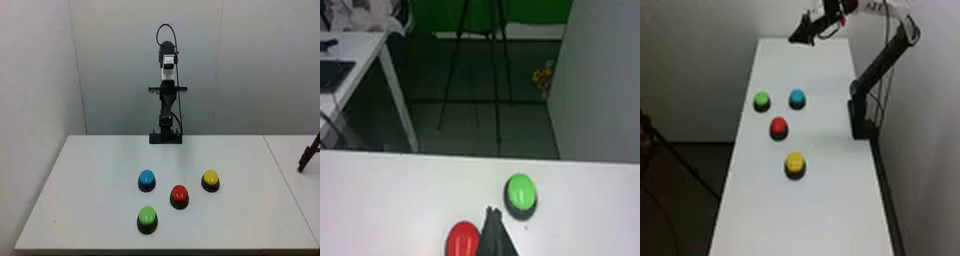
\includegraphics[width=0.8\linewidth]{figures/table30_subtask_keyframes_train/press_the_button/init.png}
\par\smallskip{\footnotesize\textbf{Stage 1.} Press the pink button.\par}
\medskip
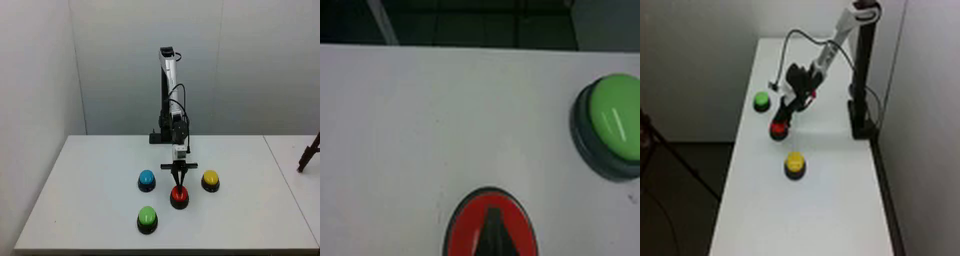
\includegraphics[width=0.8\linewidth]{figures/table30_subtask_keyframes_train/press_the_button/01_press_2.png}
\par\smallskip{\footnotesize\textbf{Stage 2.} Press the blue button.\par}
\medskip
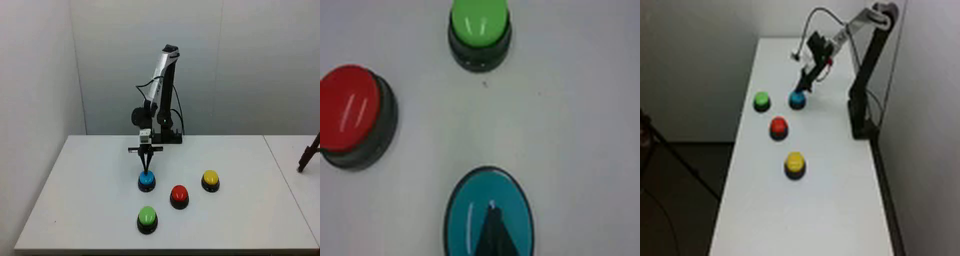
\includegraphics[width=0.8\linewidth]{figures/table30_subtask_keyframes_train/press_the_button/02_press_3.png}
\par\smallskip{\footnotesize\textbf{Stage 3.} Press the green button.\par}
\medskip
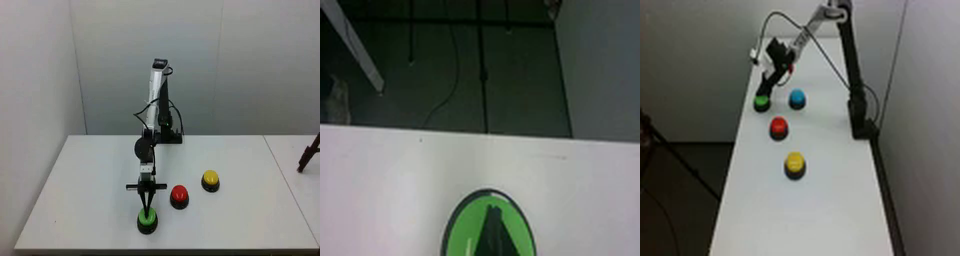
\includegraphics[width=0.8\linewidth]{figures/table30_subtask_keyframes_train/press_the_button/03_press_4.png}
\par\smallskip{\footnotesize\textbf{Stage 4.} Press the yellow button, then retract the gripper.\par}
\caption{\textbf{Button pressing (ARX5).} Subtask segmentation example. The initial observation (Stage 1) and subsequent stage observations are shown in order, each paired with its subtask instruction.}
\label{fig:subtask_press_the_button}
\end{figure}

\begin{figure}[tp]
\centering
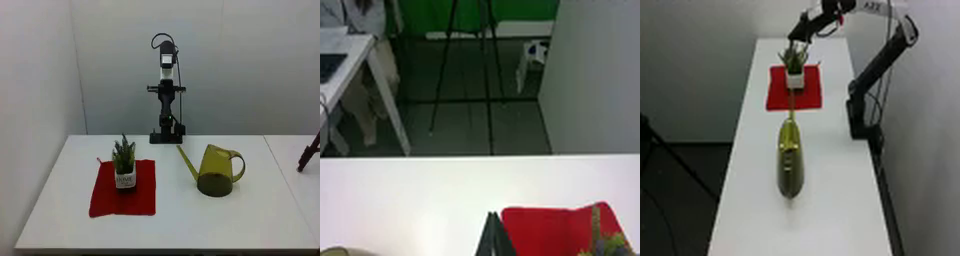
\includegraphics[width=0.8\linewidth]{figures/table30_subtask_keyframes_train/water_the_flowers/init.png}
\par\smallskip{\footnotesize\textbf{Stage 1.} Pick up the watering can and water the potted plant.\par}
\medskip
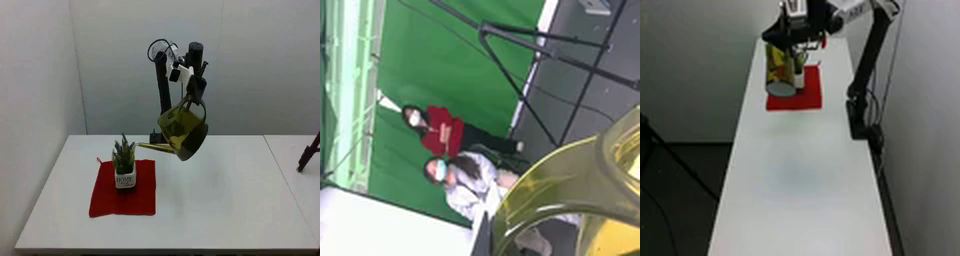
\includegraphics[width=0.8\linewidth]{figures/table30_subtask_keyframes_train/water_the_flowers/01_place.png}
\par\smallskip{\footnotesize\textbf{Stage 2.} The watering is finished, put the watering can down.\par}
\caption{\textbf{Plant watering (ARX5).} Subtask segmentation example. The initial observation (Stage 1) and subsequent stage observations are shown in order, each paired with its subtask instruction.}
\label{fig:subtask_water_the_flowers}
\end{figure}

\begin{figure}[tp]
\centering
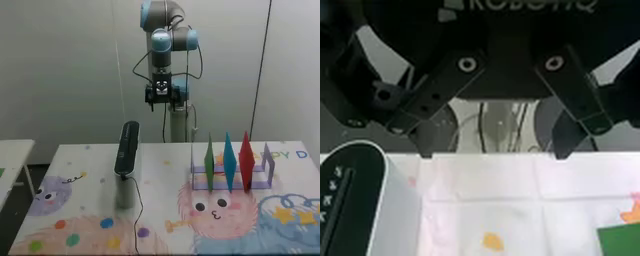
\includegraphics[width=0.8\linewidth]{figures/table30_subtask_keyframes_train/shred_paper/init.png}
\par\smallskip{\footnotesize\textbf{Stage 1.} Put the paper into the shredder.\par}
\medskip
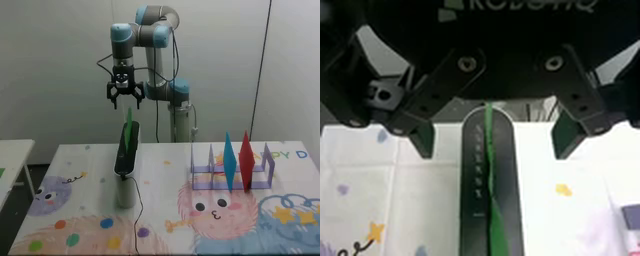
\includegraphics[width=0.8\linewidth]{figures/table30_subtask_keyframes_train/shred_paper/01_retract.png}
\par\smallskip{\footnotesize\textbf{Stage 2.} Retract gripper.\par}
\caption{\textbf{Paper shredding (UR5).} Subtask segmentation example. The initial observation (Stage 1) and subsequent stage observations are shown in order, each paired with its subtask instruction.}
\label{fig:subtask_shred_paper}
\end{figure}

\begin{figure}[tp]
\centering
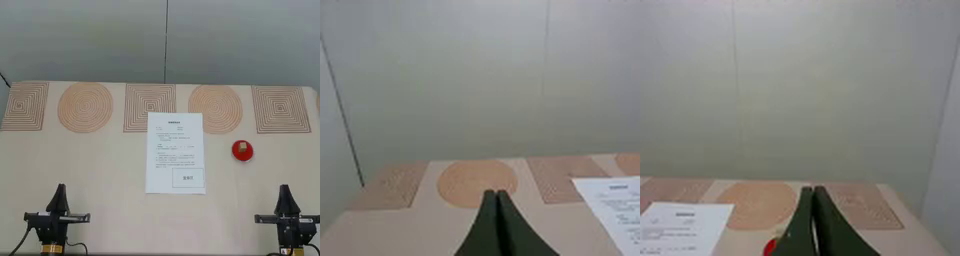
\includegraphics[width=0.8\linewidth]{figures/table30_subtask_keyframes_train/stamp_positioning/init.png}
\par\smallskip{\footnotesize\textbf{Stage 1.} Pick up the stamp.\par}
\medskip
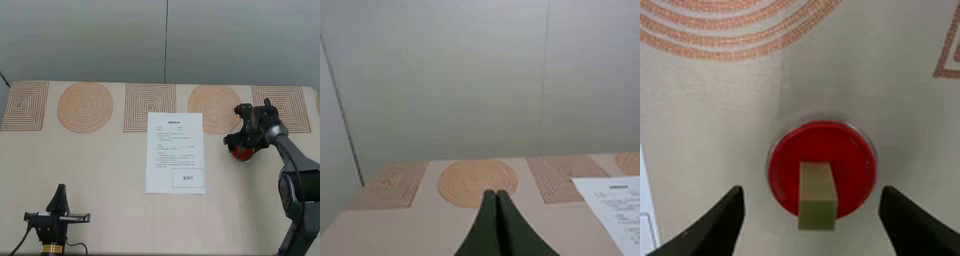
\includegraphics[width=0.8\linewidth]{figures/table30_subtask_keyframes_train/stamp_positioning/01_dip.png}
\par\smallskip{\footnotesize\textbf{Stage 2.} Dip into the ink.\par}
\medskip
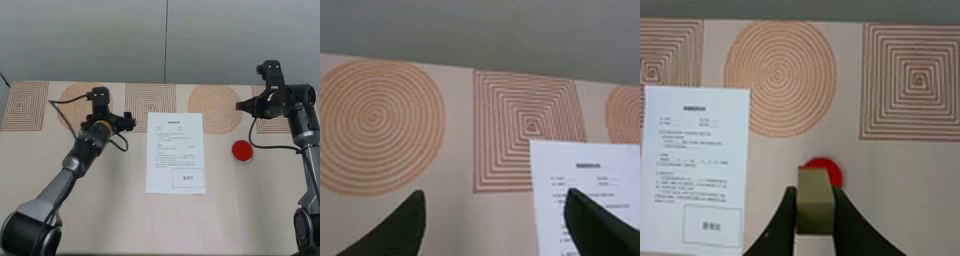
\includegraphics[width=0.8\linewidth]{figures/table30_subtask_keyframes_train/stamp_positioning/02_stamp.png}
\par\smallskip{\footnotesize\textbf{Stage 3.} Stamp the signature area and return.\par}
\caption{\textbf{Stamp positioning (ALOHA).} Subtask segmentation example. The initial observation (Stage 1) and subsequent stage observations are shown in order, each paired with its subtask instruction.}
\label{fig:subtask_stamp_positioning}
\end{figure}


\section{RoboChallenge Table30-V2 Leaderboard}
\label{app:leaderboard}
% Figure~\ref{fig:table30_leaderboard} reproduces the leaderboard snapshot associated with the reported Table30-V2 evaluation.
% LoopWAM appears in first place in this snapshot, with a score of 56.80 and a success rate of 43.33\%.
Figure~\ref{fig:table30_leaderboard} presents the official RoboChallenge Table30-V2 leaderboard at the time of evaluation.
LoopWAM ranks first, achieving an overall score of 56.80 and a success rate of 43.33\%.

\begin{figure}[t]
\centering
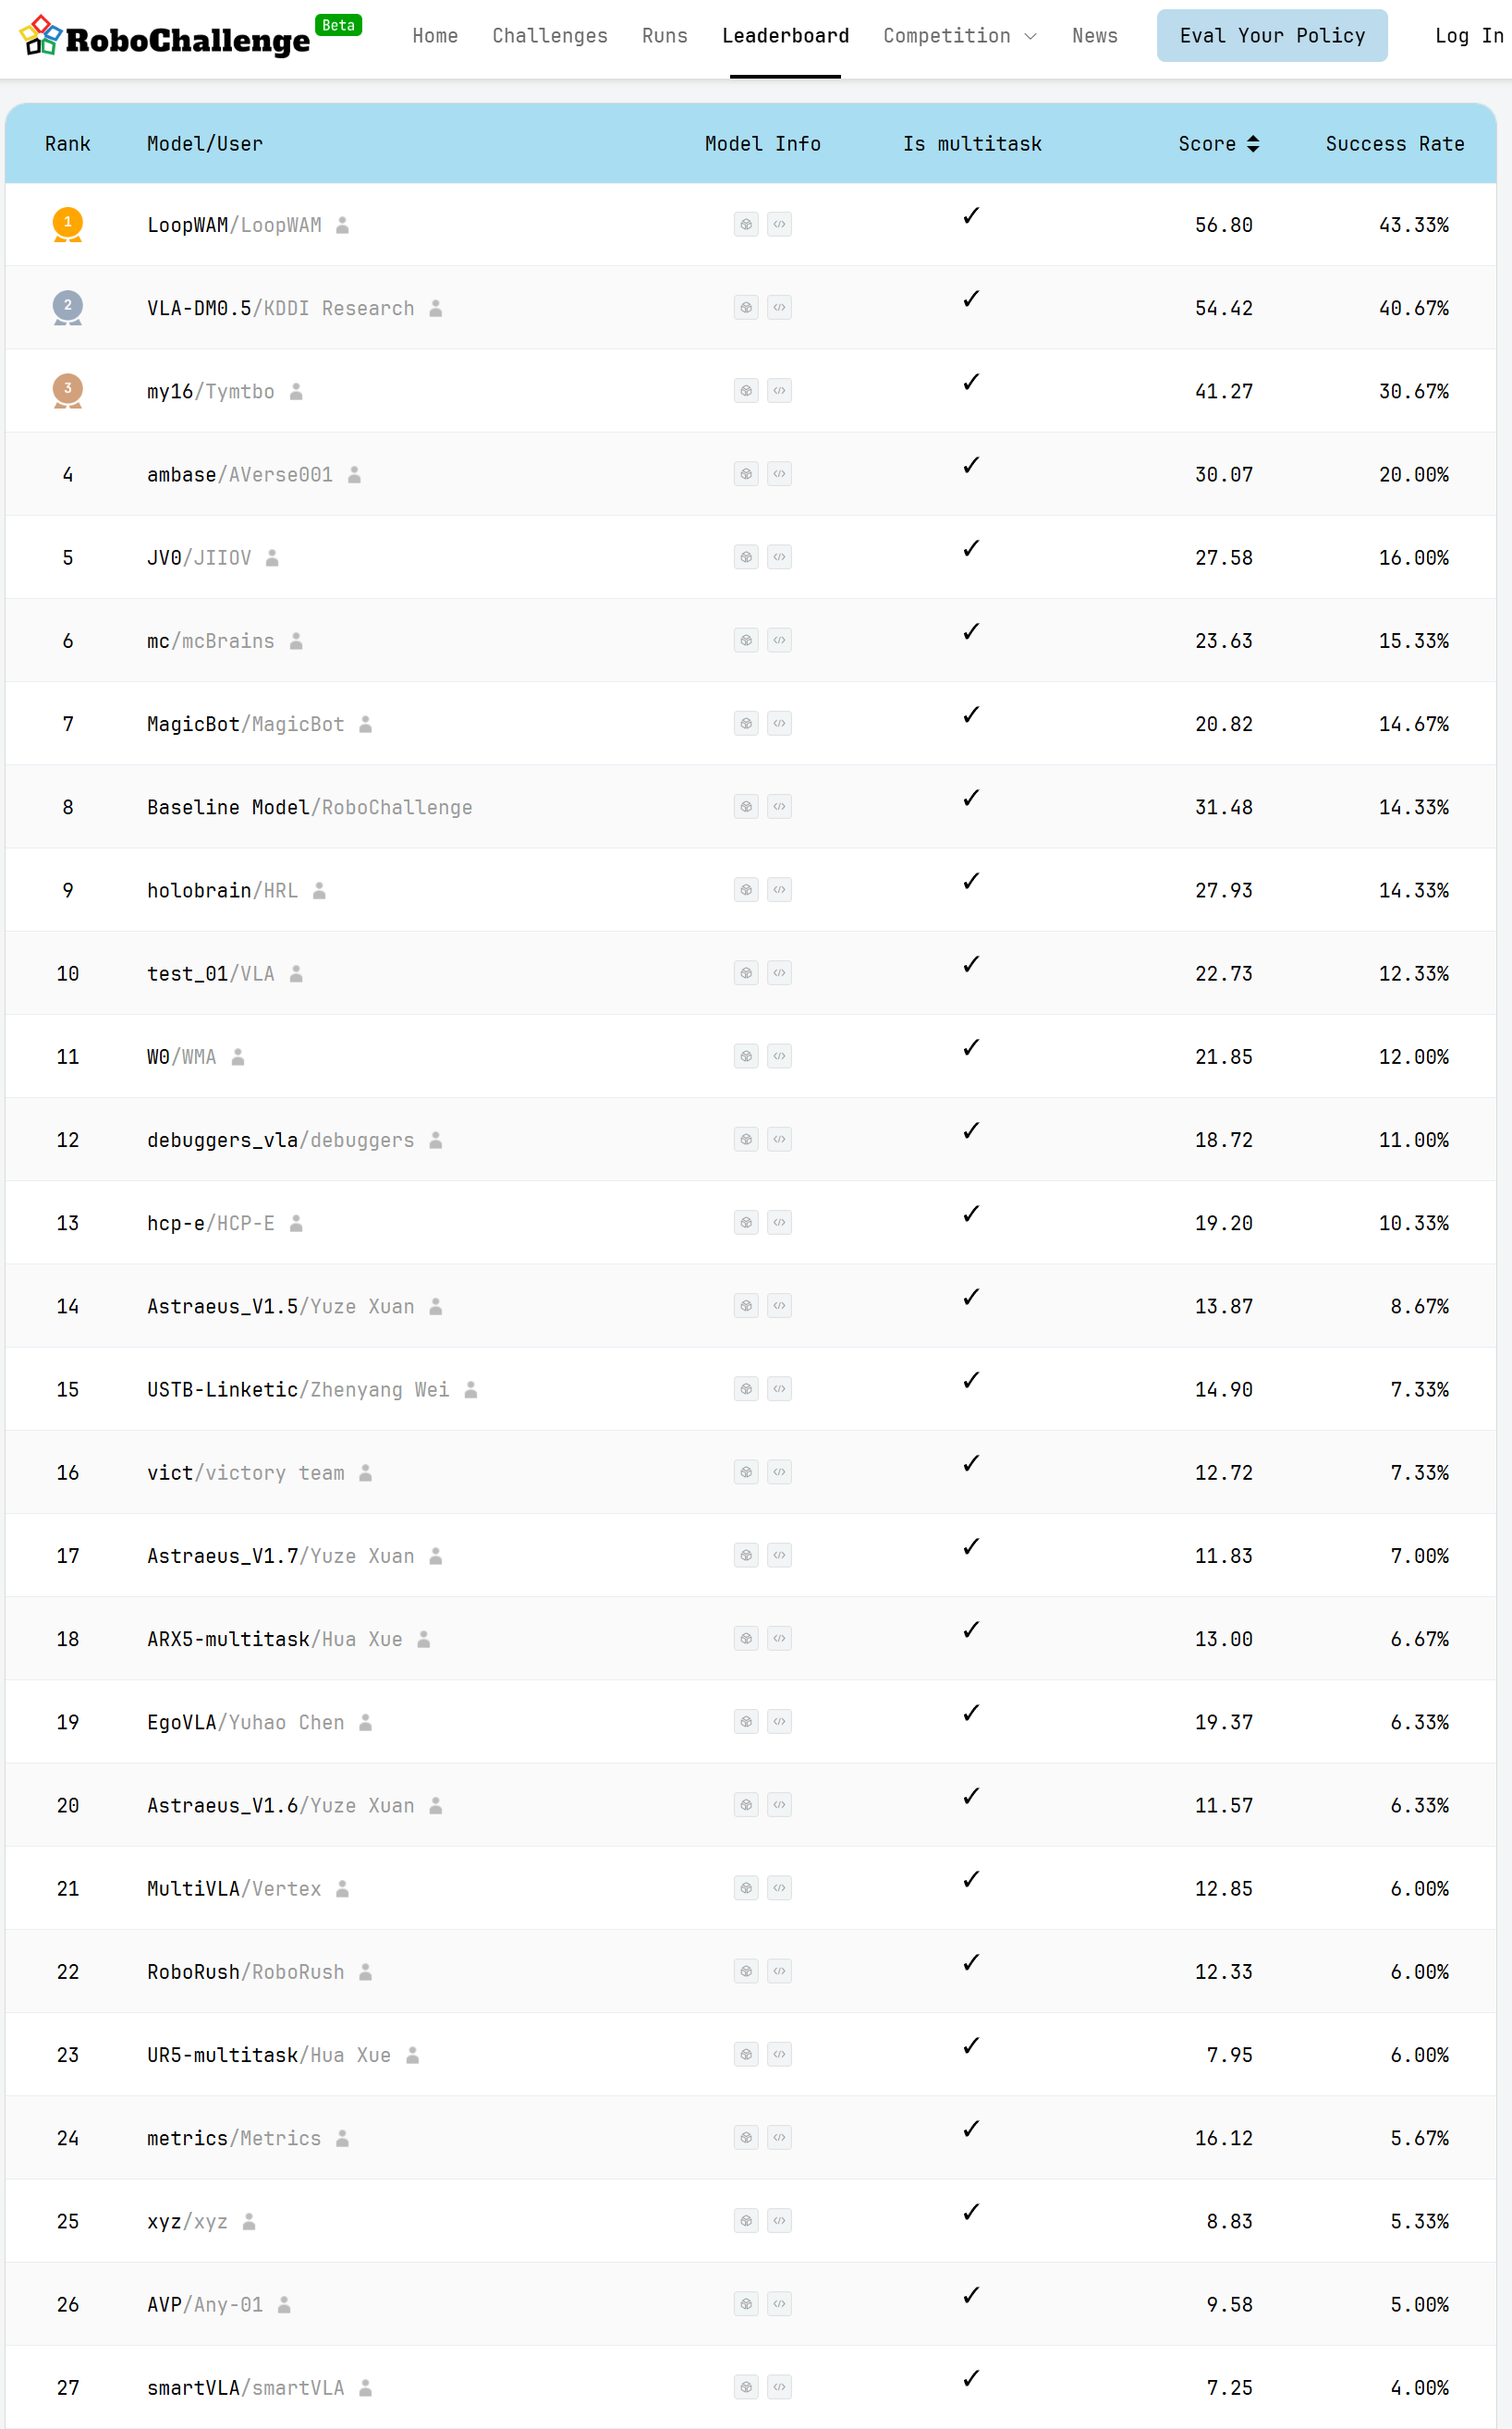
\includegraphics[width=0.82\linewidth]{figures/table30v2-leaderboard.png}
\caption{\textbf{RoboChallenge Table30-V2 leaderboard.} LoopWAM ranks first with an overall score of 56.80 and a success rate of 43.33\%, using a multi-task policy for each embodiment.}
\label{fig:table30_leaderboard}
\end{figure}

\section{Failure Recovery and Iterative Execution}
\label{app:retry}

Real-world robot manipulation often involves uncertainty caused by
imperfect perception, inaccurate execution, and complex object
interaction dynamics.

To analyze the ability of LoopWAM to support iterative execution,
Figure~\ref{fig:retry_success} presents qualitative examples where an
initial attempt does not complete the desired task.

After observing the resulting environment state, the model generates
subsequent corrective behaviors that improve the execution outcome.
These examples highlight the importance of modeling future states and
environment transitions beyond predicting isolated actions.


\begin{figure}[t]
    \centering

    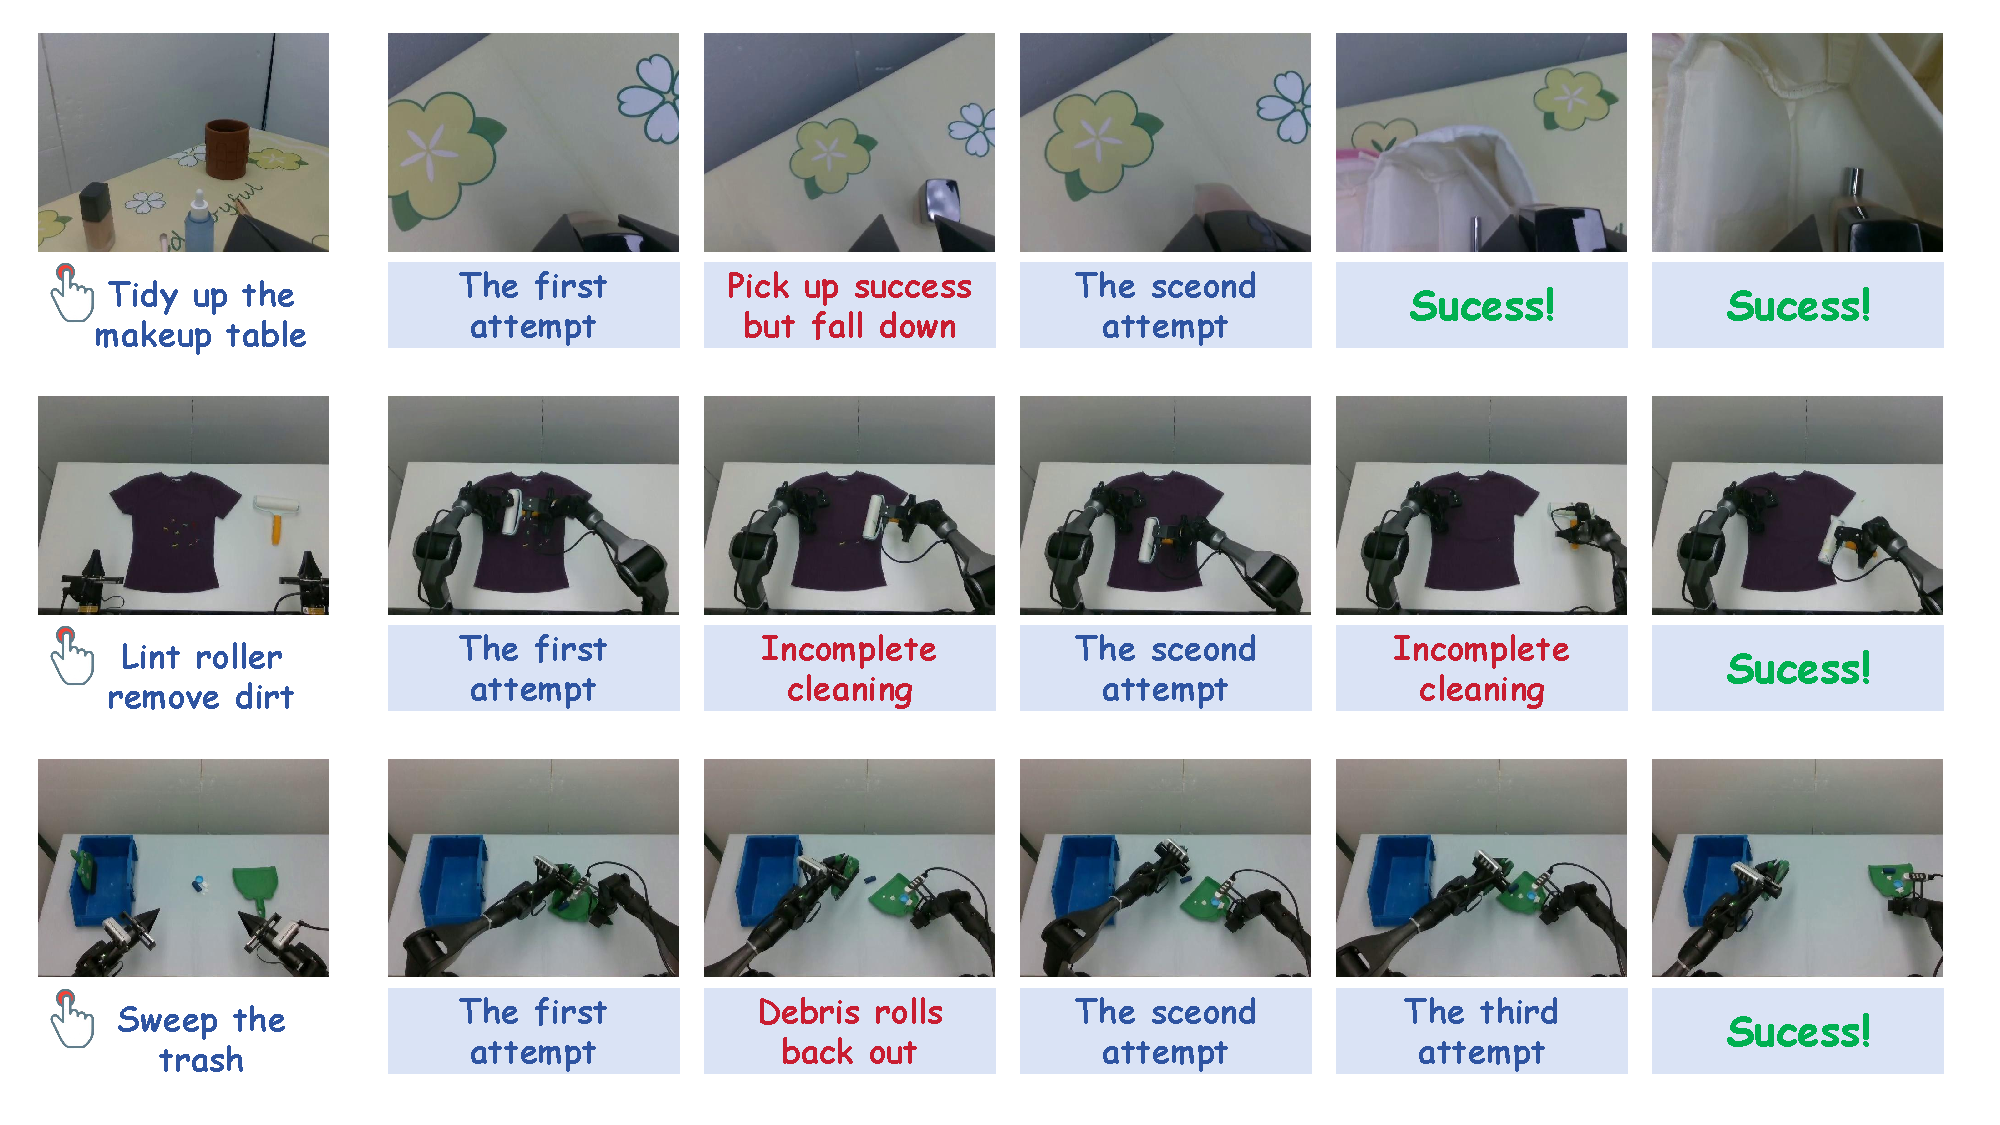
\includegraphics[width=\linewidth]{figures/lyp/retry-sucess.pdf}

    \caption{
        Qualitative examples of iterative execution and failure recovery.
        The first attempt may fail due to execution uncertainty,
        incomplete interaction, or object displacement.
        Subsequent attempts generate corrective behaviors and achieve
        successful task completion.
    }
    \label{fig:retry_success}
\end{figure}




\section{Qualitative Future Observation Prediction}
\label{app:video_prediction}

As a learned robot world model, LoopWAM predicts future visual
observations conditioned on the current robot state and interaction
history.

To further examine the learned visual dynamics,
Figure~\ref{fig:video_prediction} compares predicted future frames with
ground-truth observations from robot executions.

The predictions capture major aspects of scene evolution, including
robot motion, object movement, and manipulation progress.
Although generated observations may differ from the ground-truth images
in fine visual details, they preserve the temporal structure of the
interaction process.


\begin{figure}[t]
    \centering

    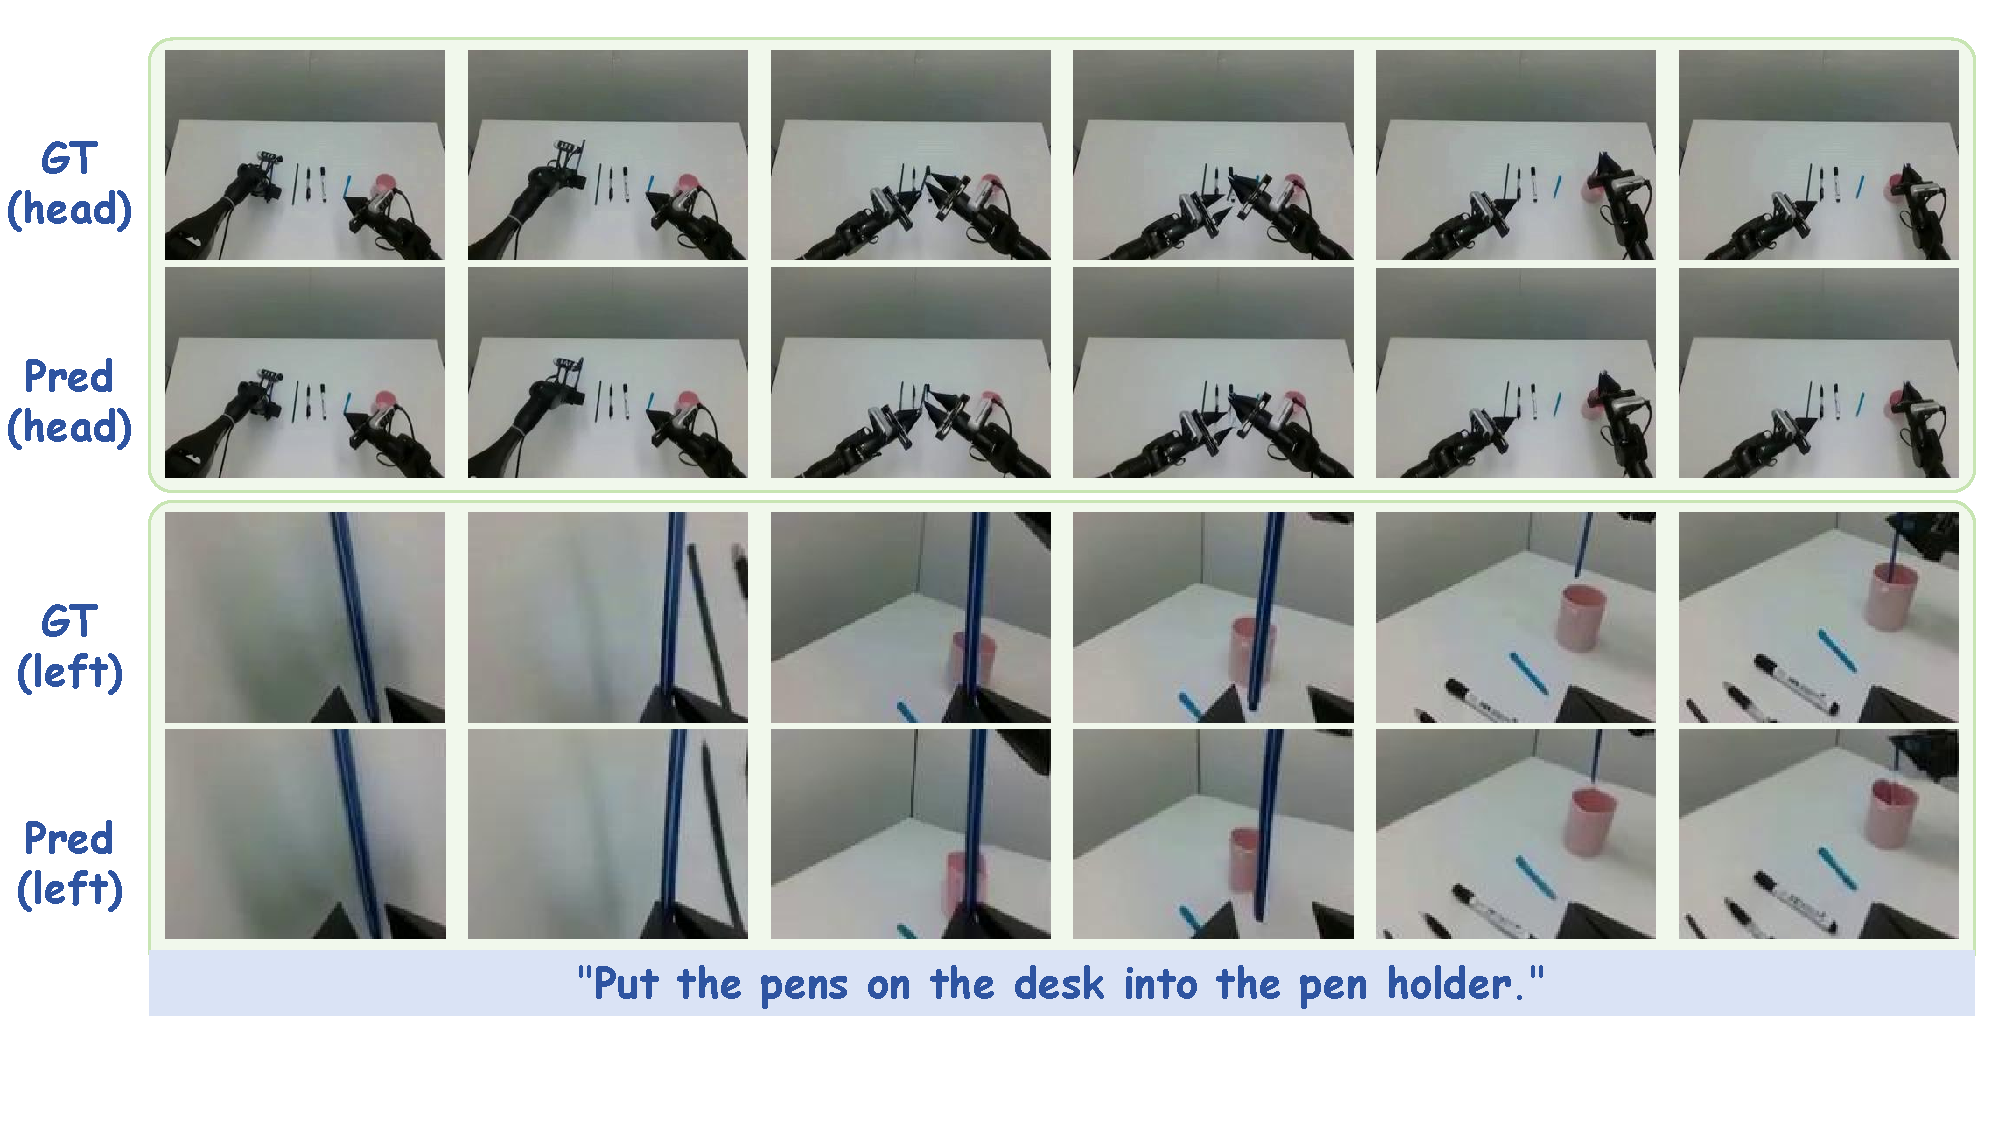
\includegraphics[width=\linewidth]{figures/lyp/video-pred-1.pdf}

    \vspace{0.5em}

    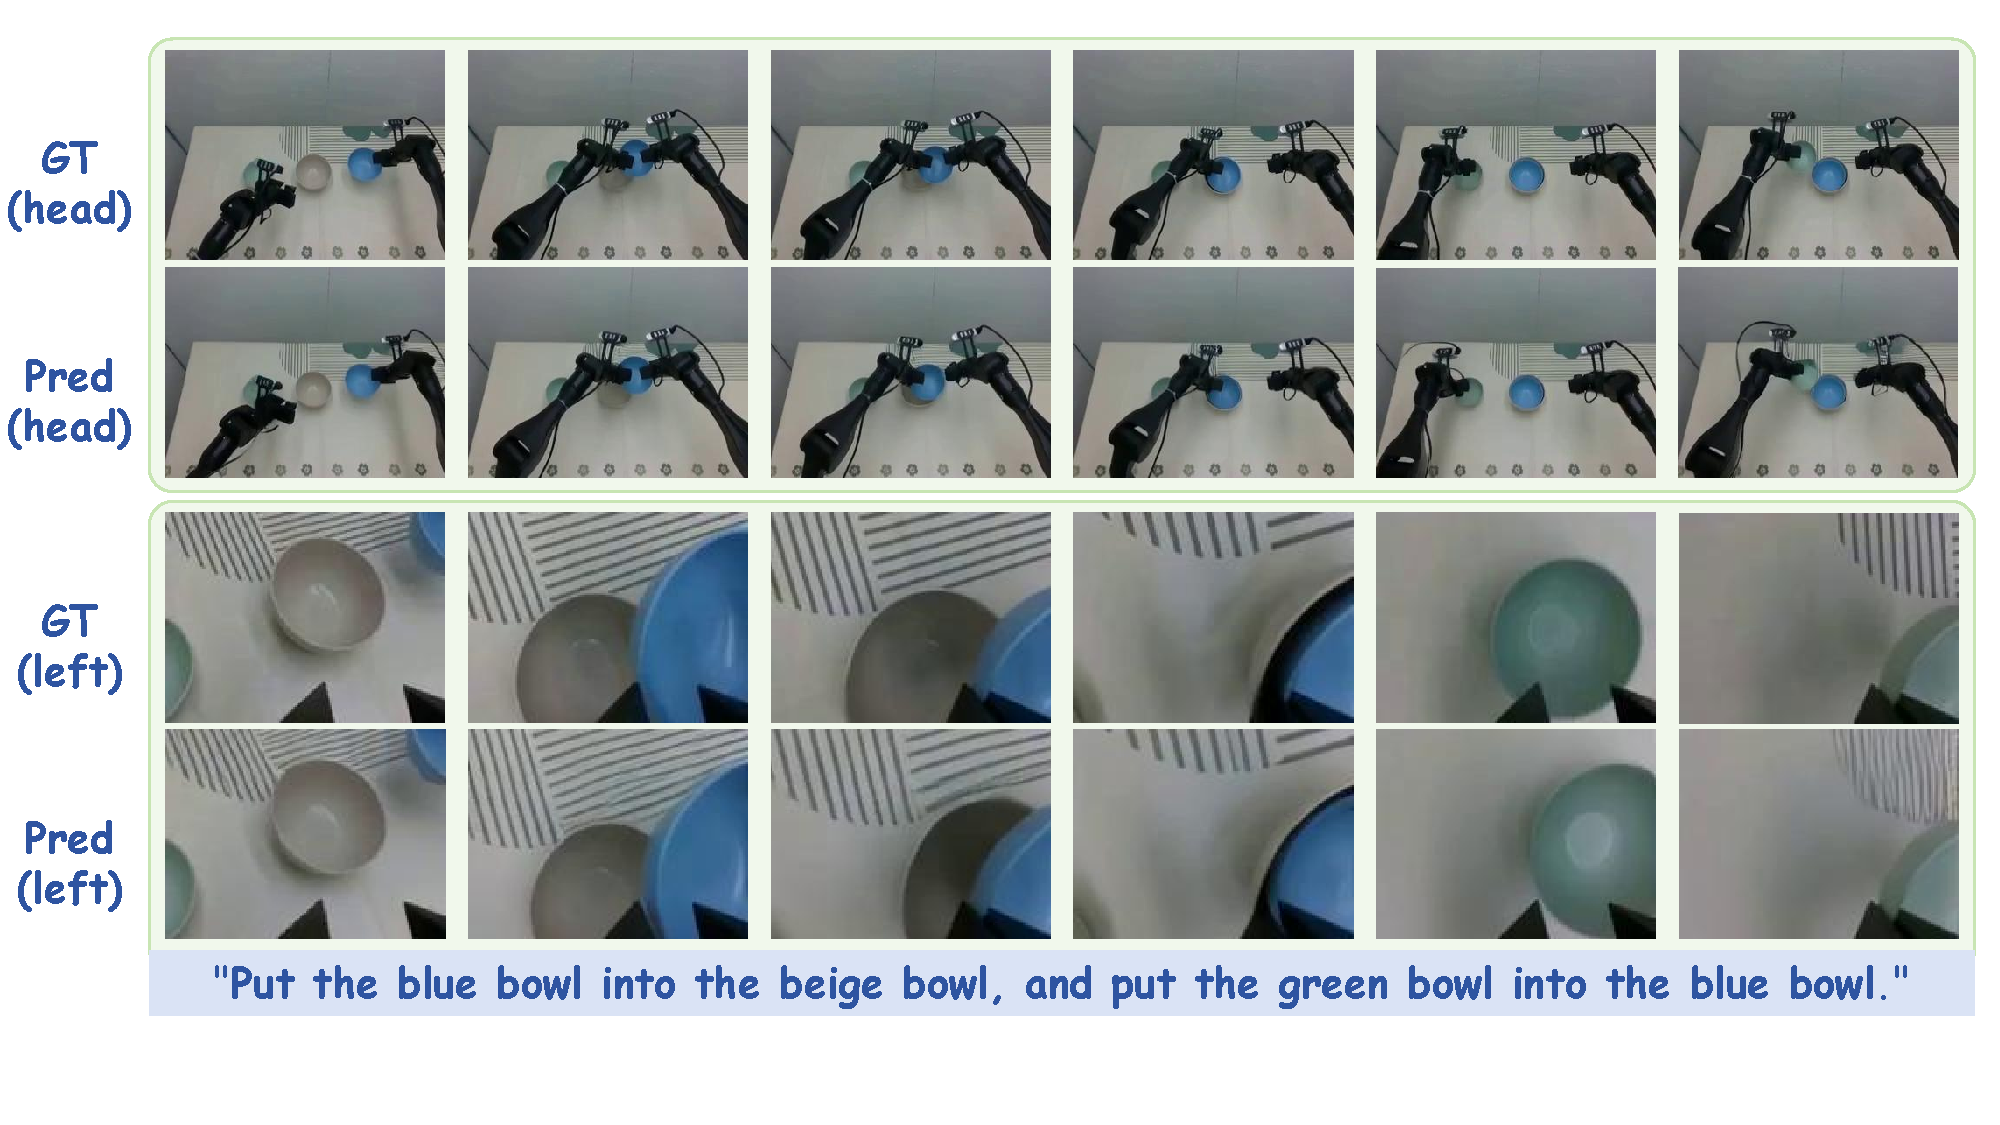
\includegraphics[width=\linewidth]{figures/lyp/video-pred-2.pdf}

    \caption{
        Qualitative comparison between predicted future observations from
        LoopWAM and ground-truth robot executions.
        The model captures the temporal evolution of robot-object
        interactions and predicts plausible future visual states.
    }
    \label{fig:video_prediction}
\end{figure}


\section{Representative Robot Platforms and Tasks}
\label{app:robot_tasks}

LoopWAM is evaluated across multiple robot platforms with different
embodiments, sensing configurations, and manipulation spaces.

To demonstrate the diversity of learned robot behaviors, we provide
additional qualitative examples from ARX, ALOHA, UR5, and W1 platforms.
The examples cover object manipulation, coordinated control,
fine-grained interaction, and long-horizon tasks.

Figure~\ref{fig:arx_tasks} shows representative tasks on the ARX platform.
Figure~\ref{fig:aloha_tasks} presents examples from the ALOHA platform,
which includes coordinated manipulation behaviors.
Figure~\ref{fig:ur5_tasks} demonstrates single-arm manipulation tasks on
the UR5 platform.
Finally, Figure~\ref{fig:w1_tasks} presents representative long-horizon
tasks from the W1 platform.



% ============================================================
% ARX
% ============================================================

\begin{figure}[t]
    \centering

    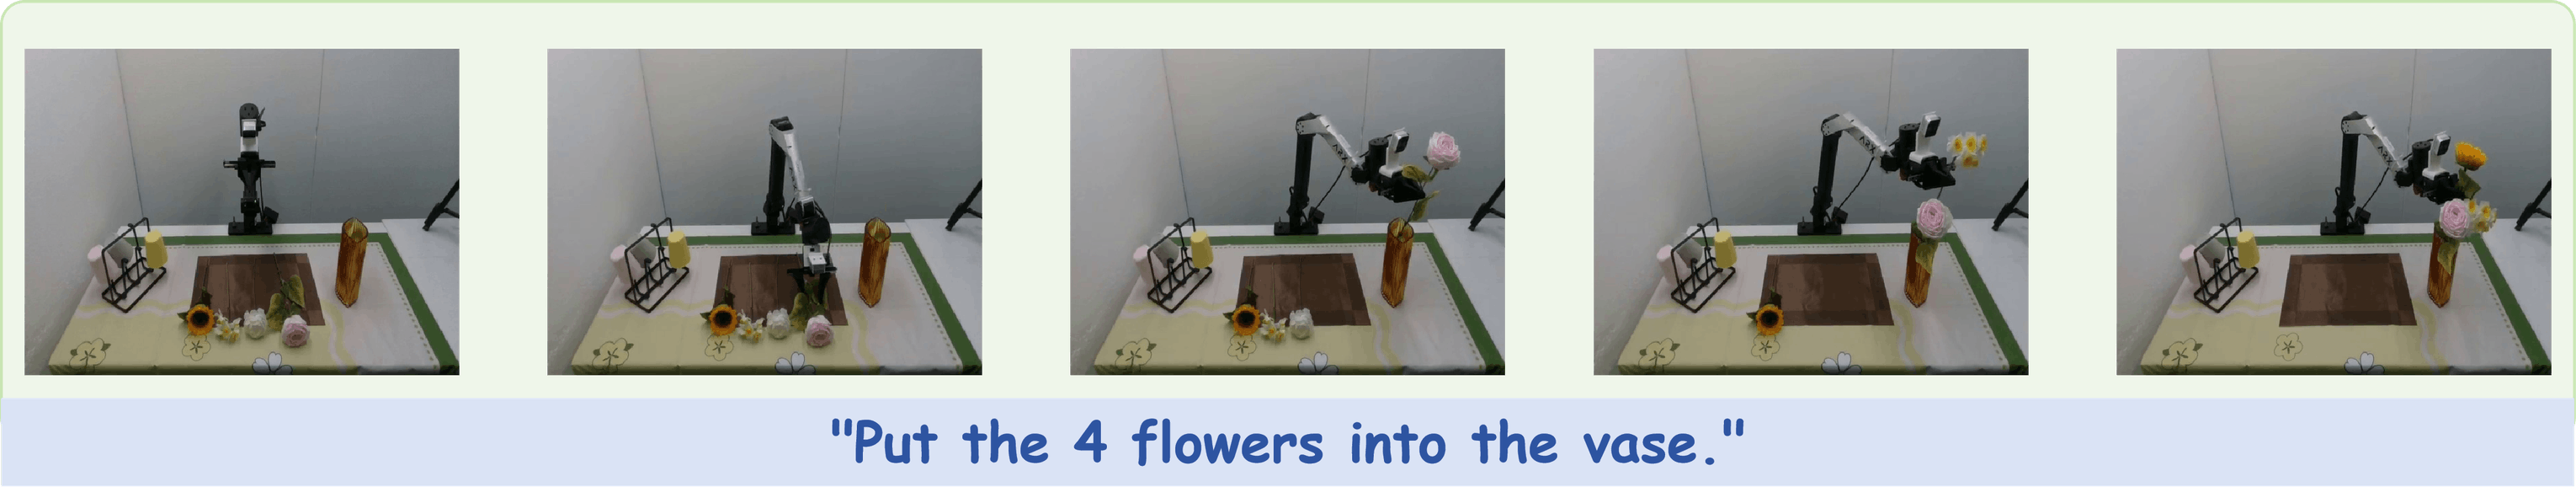
\includegraphics[width=0.95\linewidth]{figures/lyp/arx-01.png}

    \vspace{0.4em}

    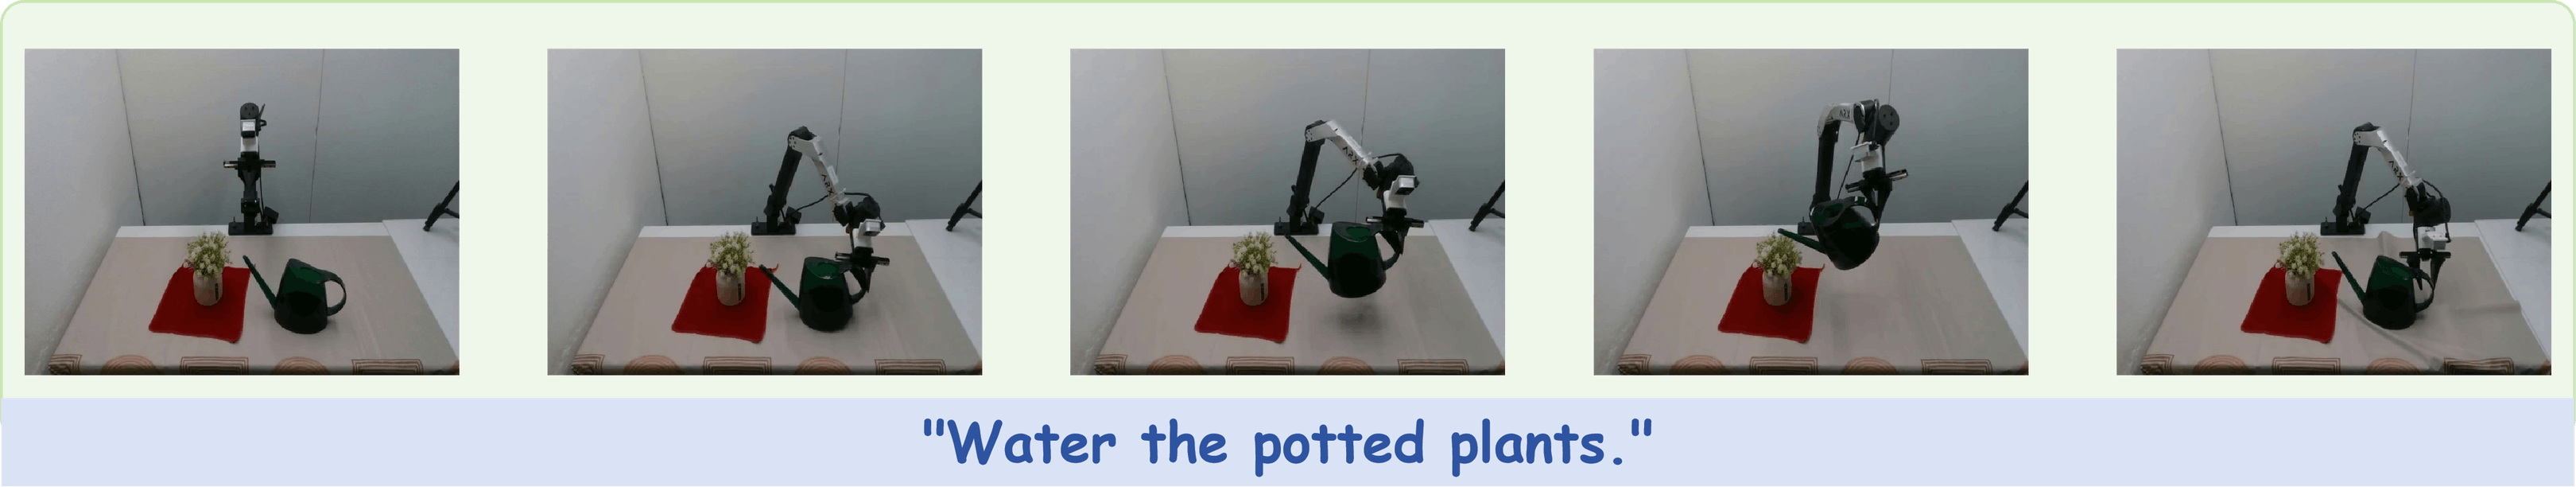
\includegraphics[width=0.95\linewidth]{figures/lyp/arx-02.png}

    \caption{
        Representative tasks on the ARX robot platform.
        The examples illustrate diverse manipulation scenarios used for
        evaluating LoopWAM across different robot embodiments.
    }
    \label{fig:arx_tasks}
\end{figure}



% ============================================================
% ALOHA
% ============================================================

\begin{figure}[t]
    \centering

    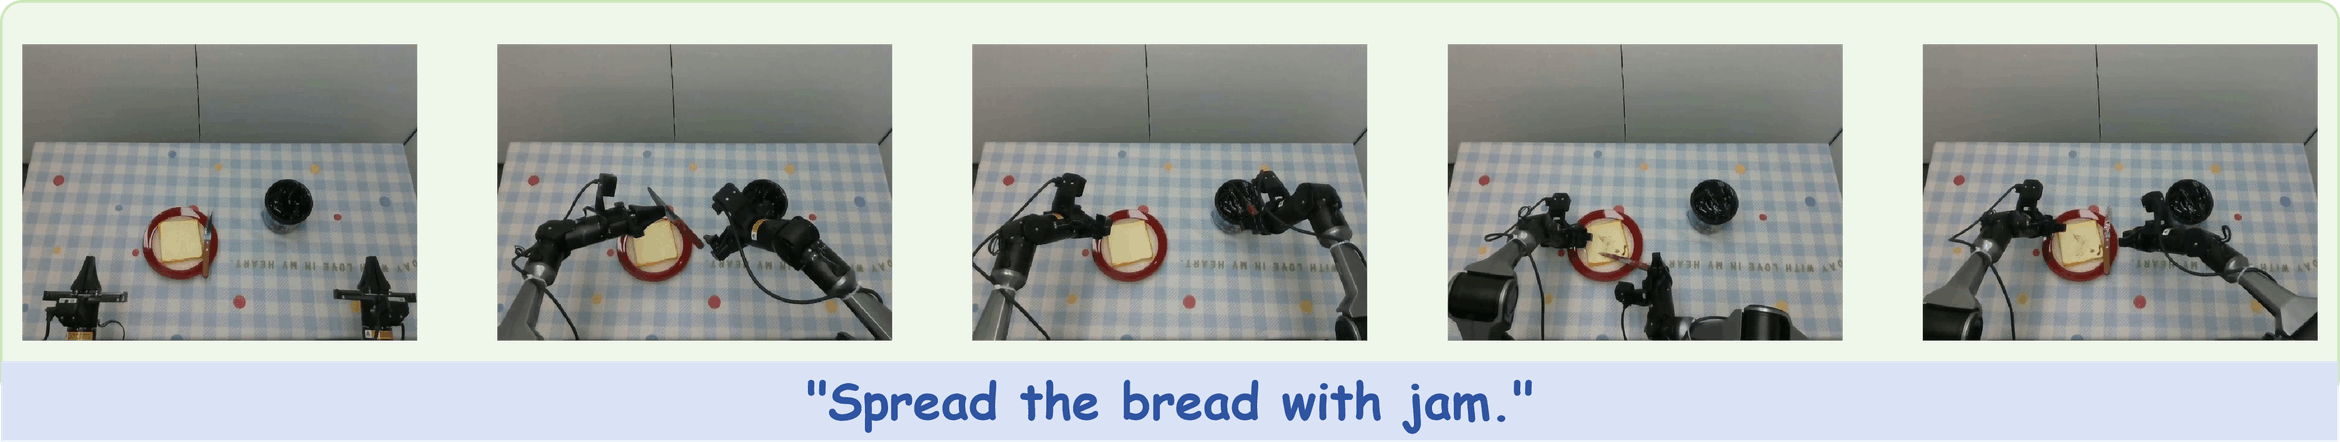
\includegraphics[width=0.95\linewidth]{figures/lyp/aloha-01.png}

    \vspace{0.4em}

    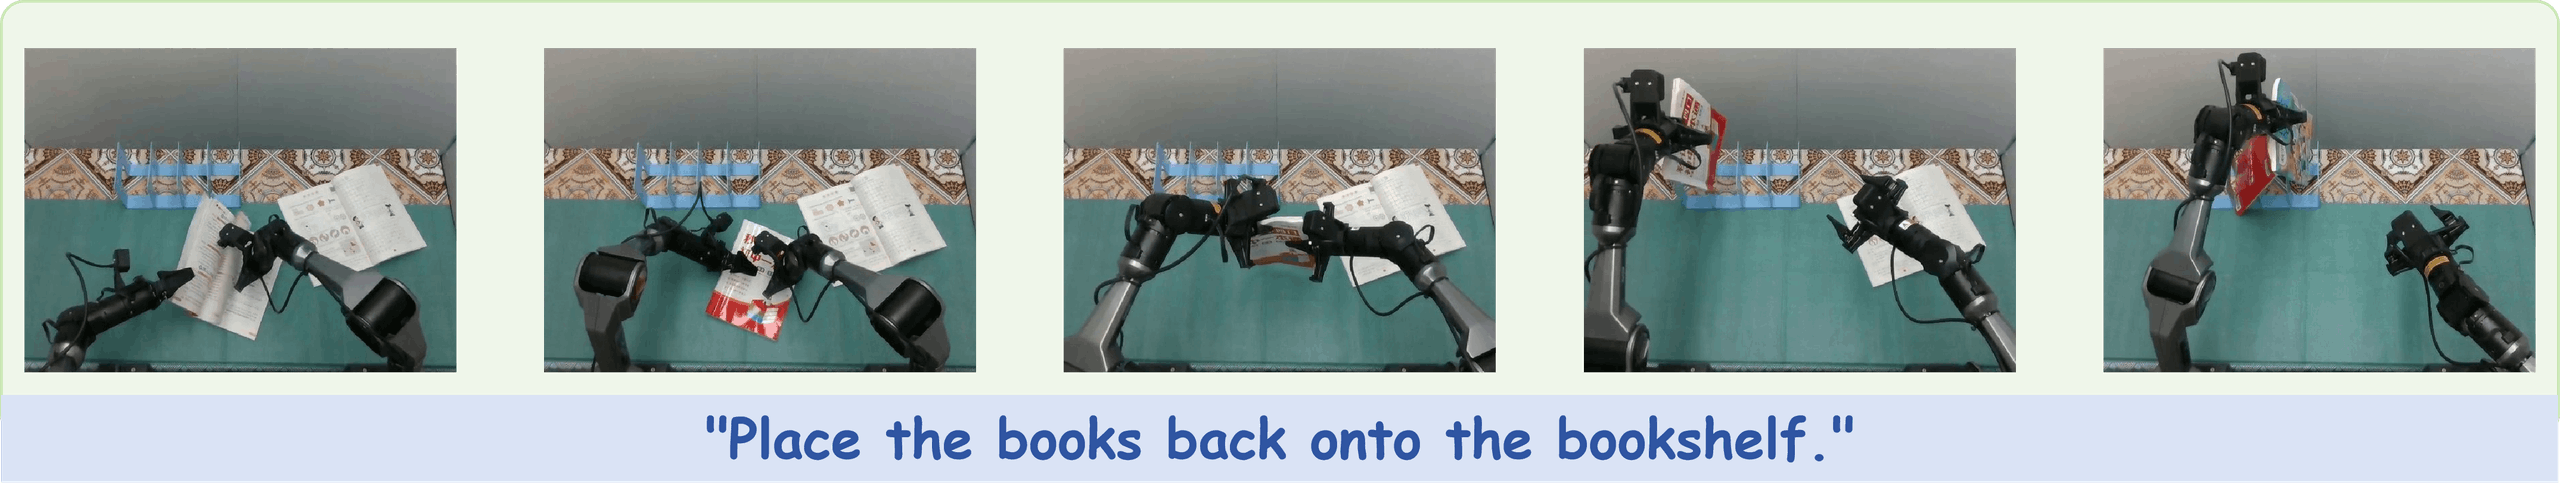
\includegraphics[width=0.95\linewidth]{figures/lyp/aloha-02.png}

    \vspace{0.4em}

    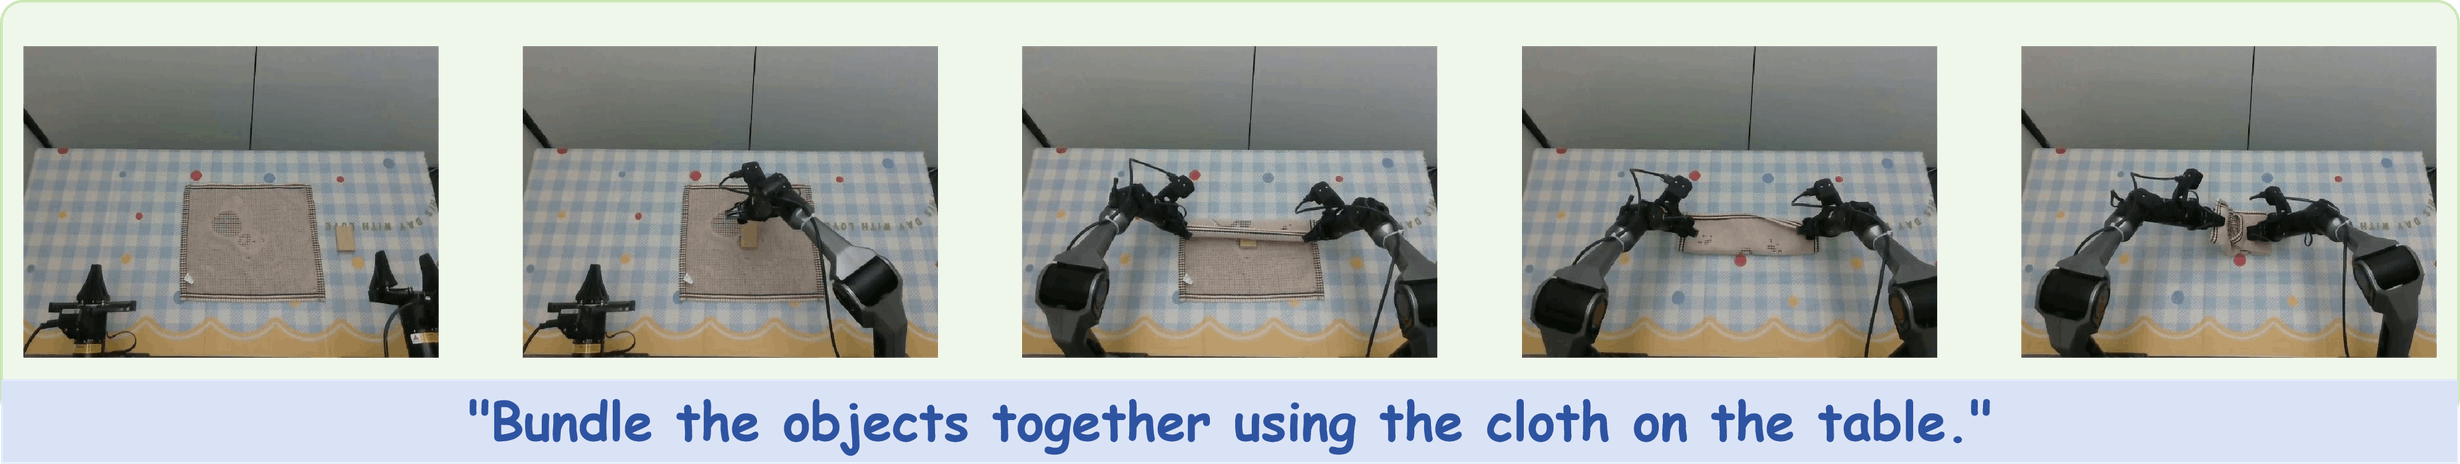
\includegraphics[width=0.95\linewidth]{figures/lyp/aloha-03.png}

    \vspace{0.4em}

    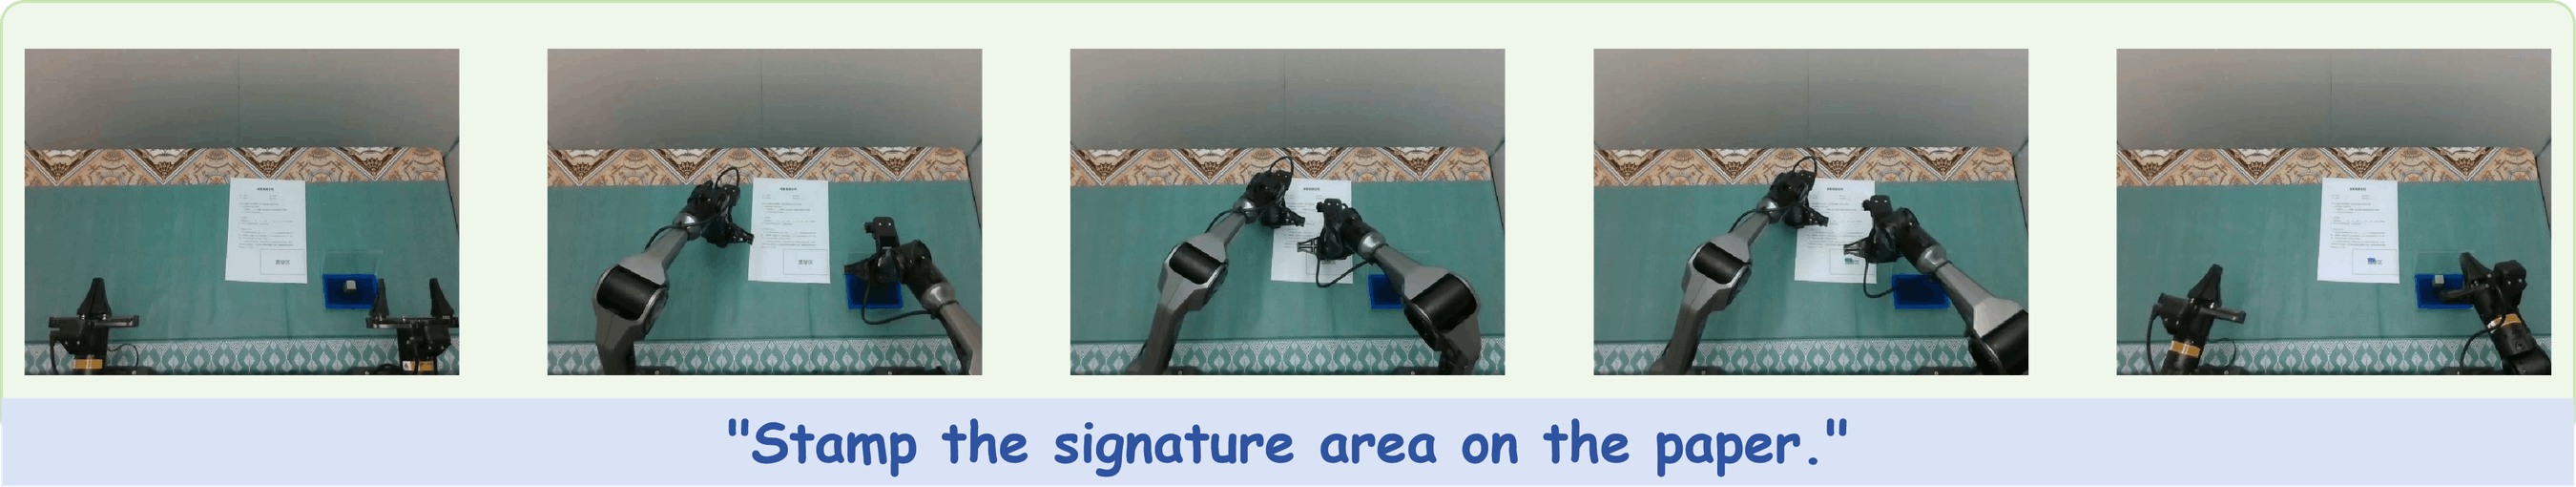
\includegraphics[width=0.95\linewidth]{figures/lyp/aloha-04.png}

    \caption{
        Representative tasks on the ALOHA robot platform.
        The examples include coordinated manipulation and object
        interaction requiring temporally consistent control.
    }
    \label{fig:aloha_tasks}
\end{figure}



% ============================================================
% UR5
% ============================================================

\begin{figure}[t]
    \centering

    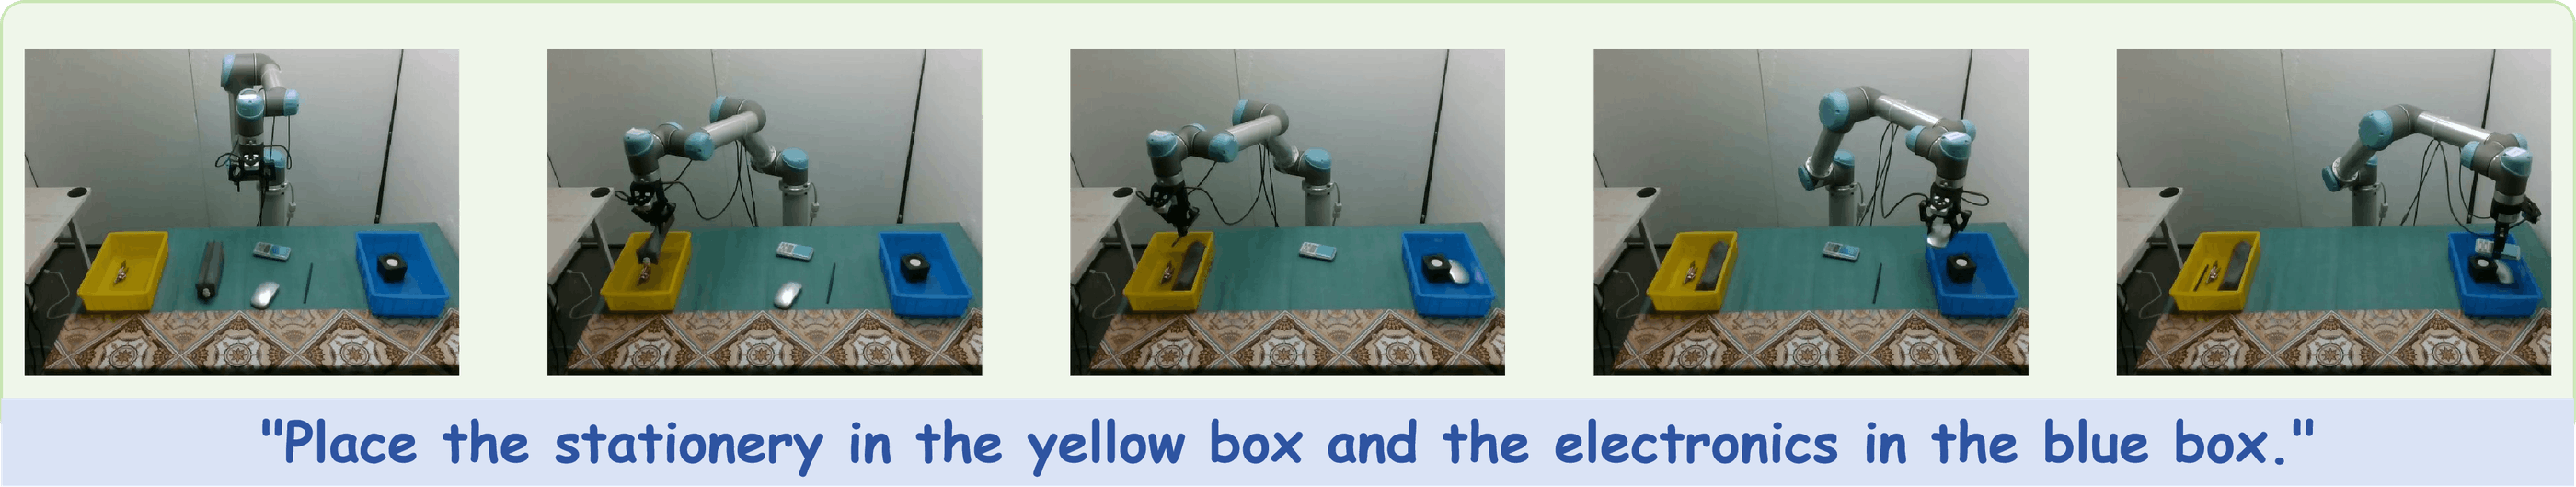
\includegraphics[width=0.95\linewidth]{figures/lyp/ur5-01.png}

    \vspace{0.4em}

    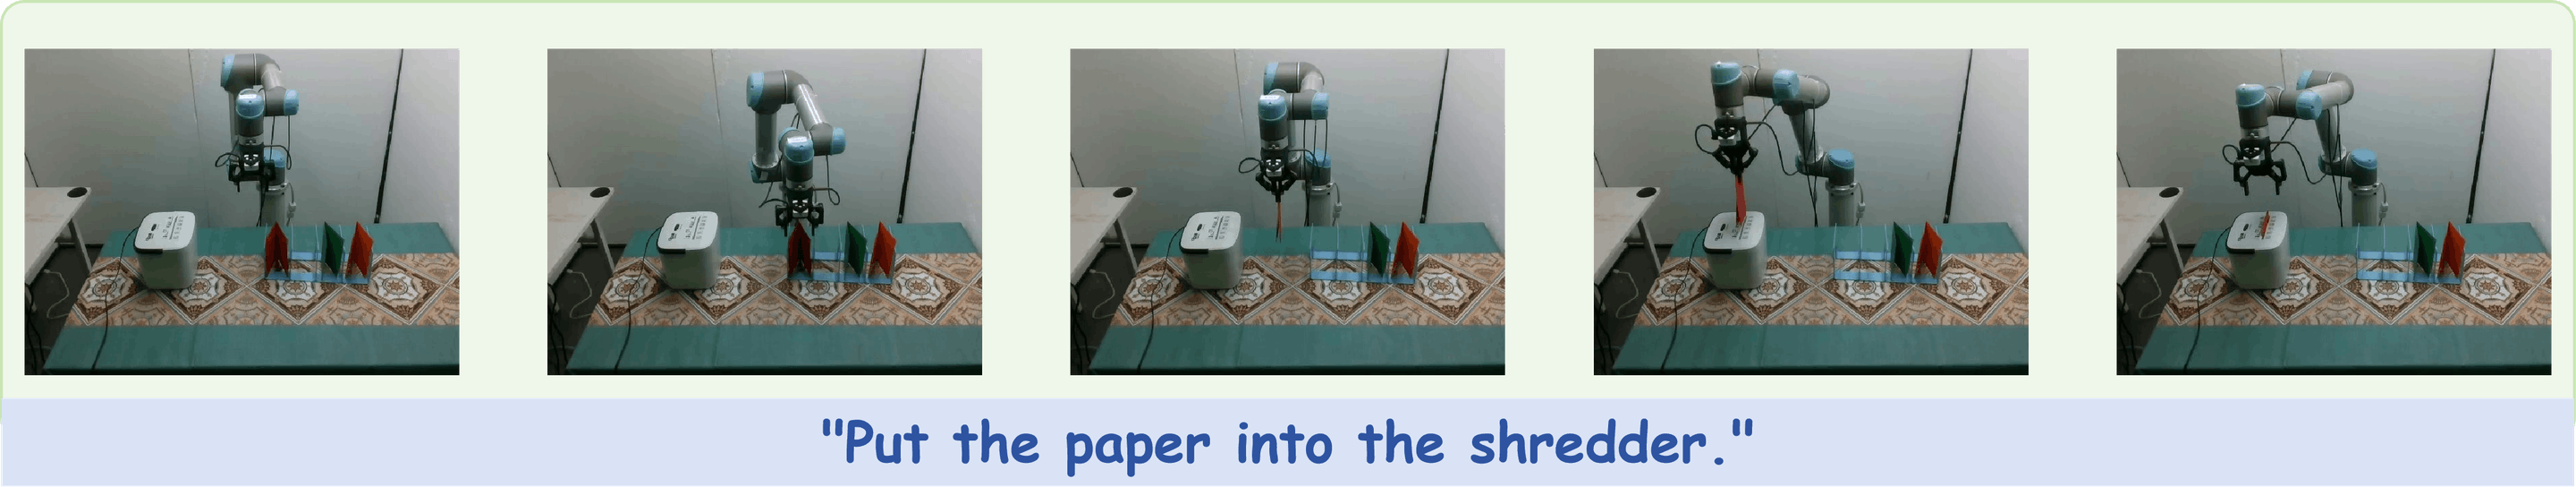
\includegraphics[width=0.95\linewidth]{figures/lyp/ur5-02.png}

    \caption{
        Representative tasks on the UR5 robot platform.
        The examples demonstrate single-arm manipulation in structured
        environments.
    }
    \label{fig:ur5_tasks}
\end{figure}



% ============================================================
% W1
% ============================================================

\begin{figure}[t]
    \centering

    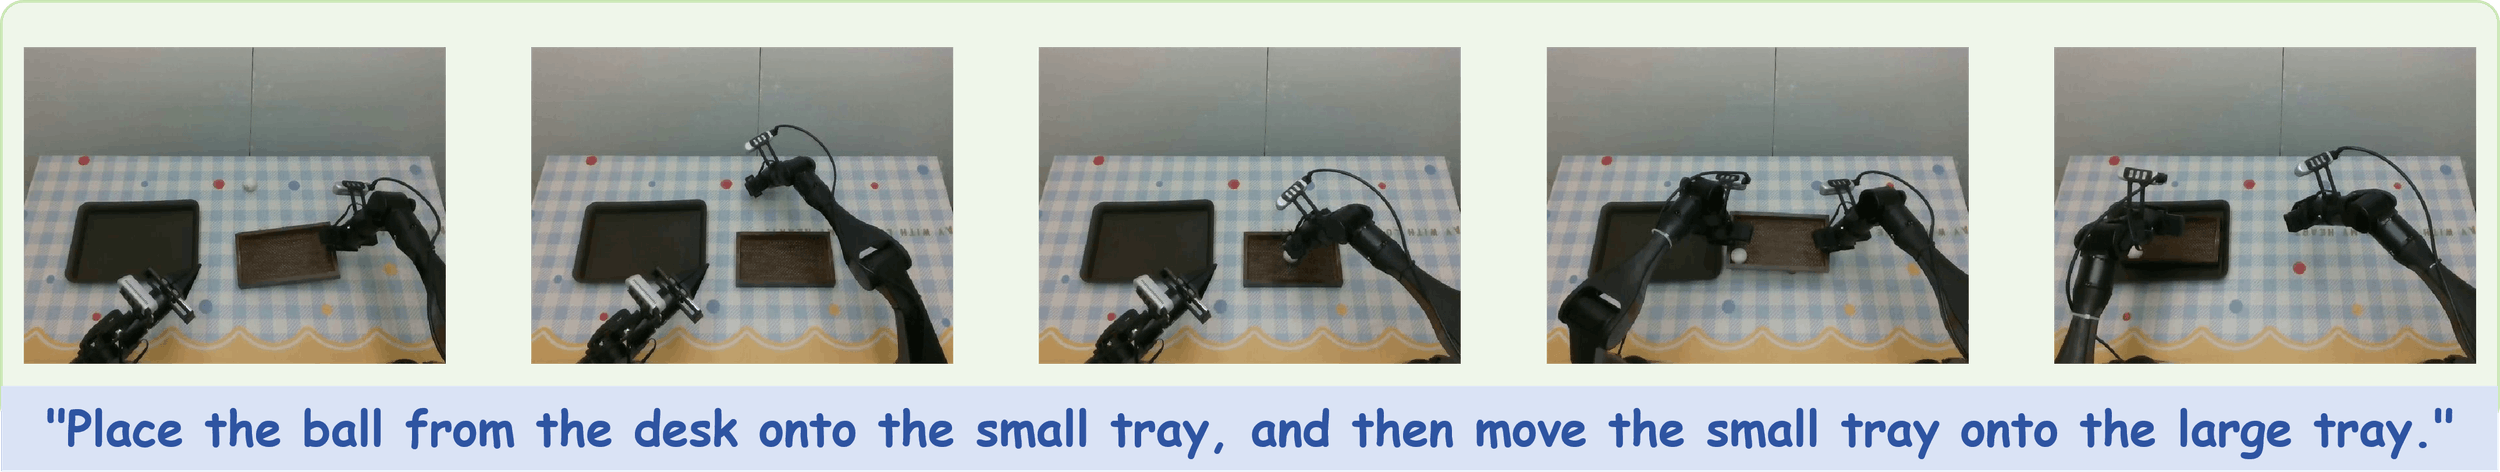
\includegraphics[width=0.95\linewidth]{figures/lyp/w1-01.png}

    \vspace{0.4em}

    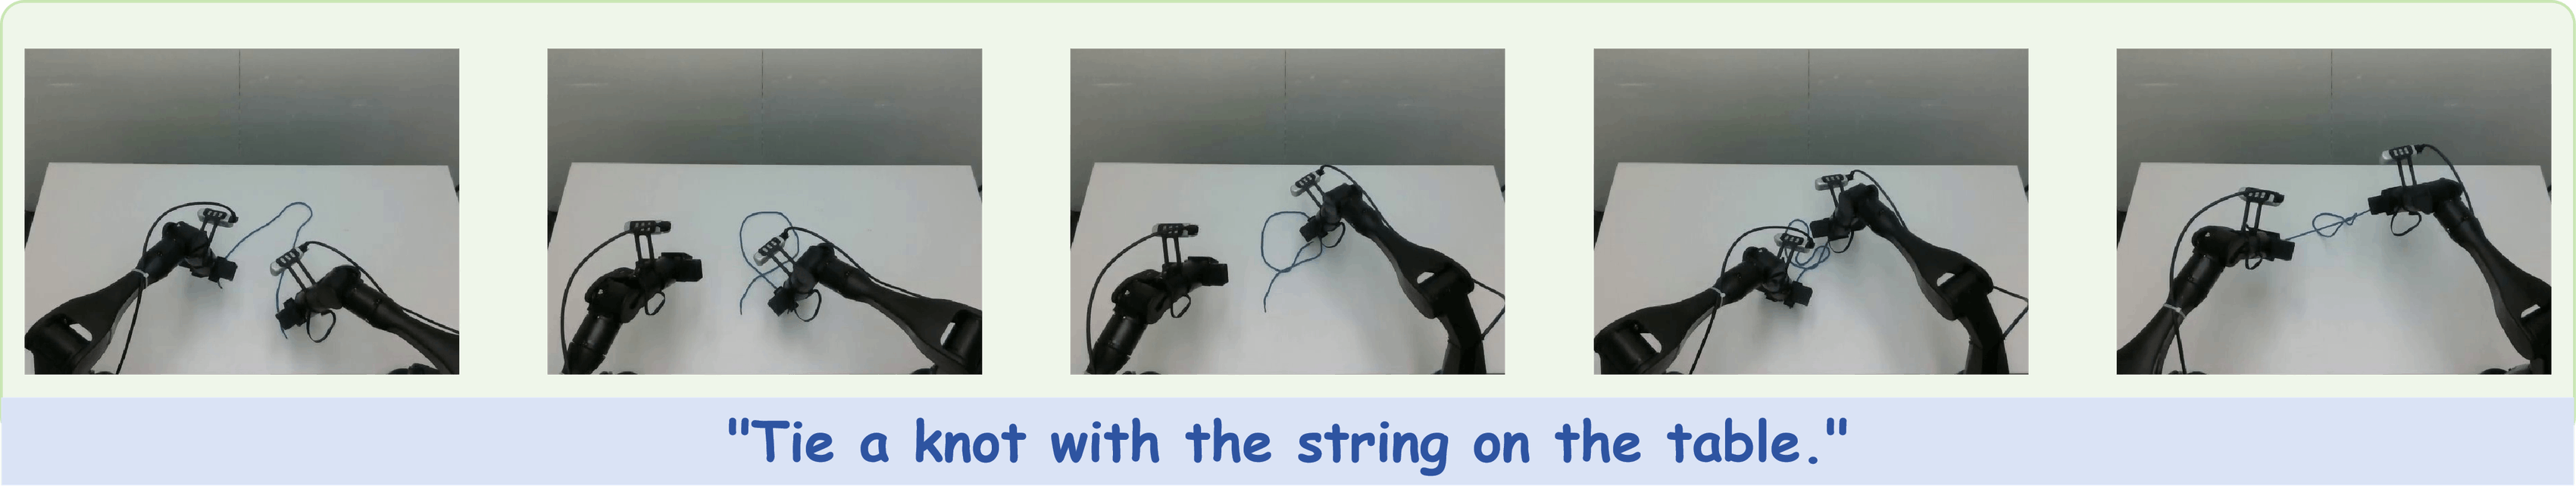
\includegraphics[width=0.95\linewidth]{figures/lyp/w1-02.png}

    \vspace{0.4em}

    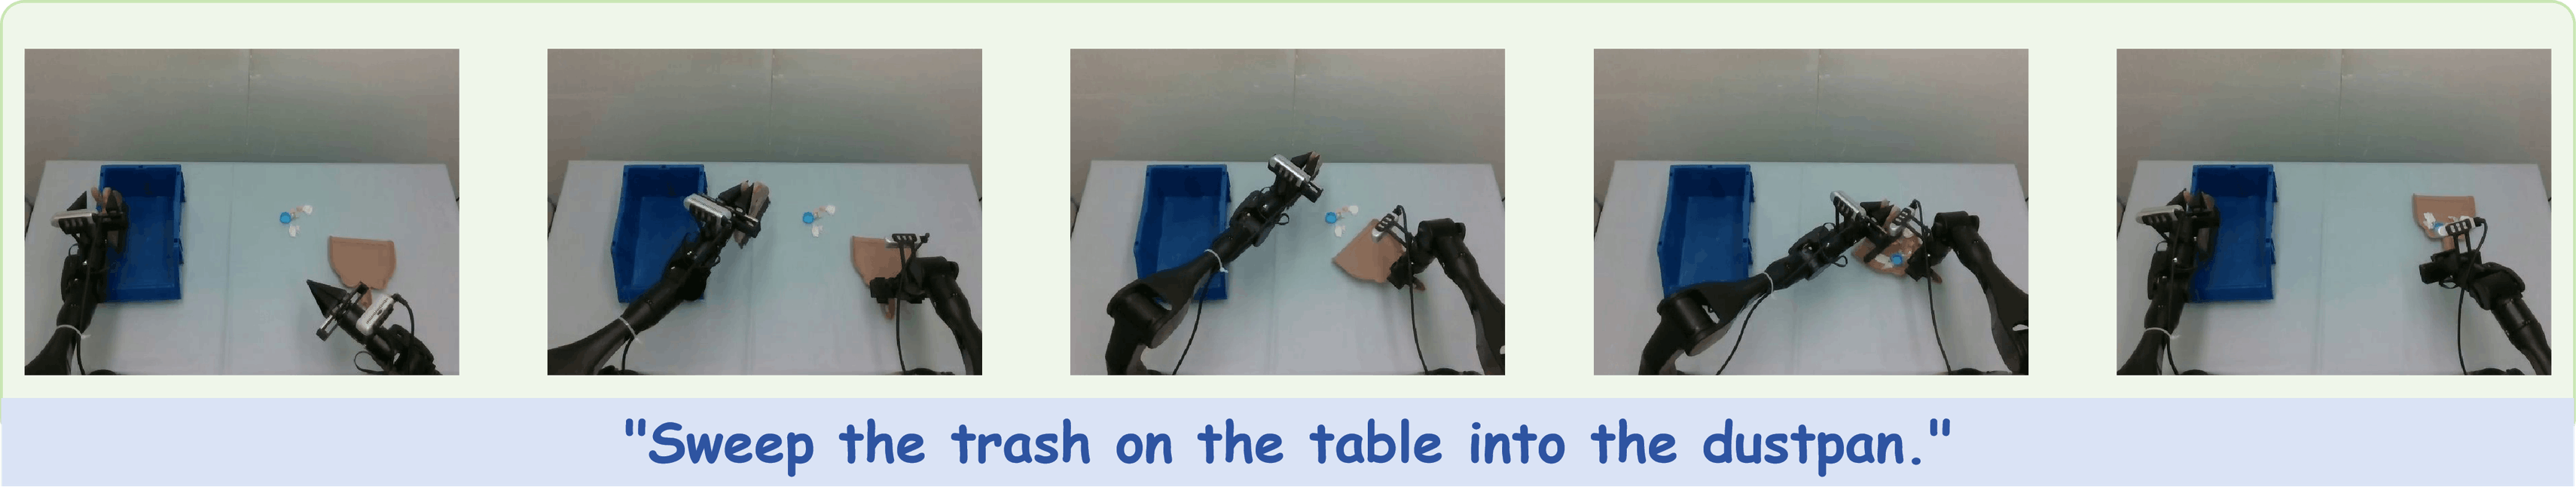
\includegraphics[width=0.95\linewidth]{figures/lyp/w1-03.png}

    \vspace{0.4em}

    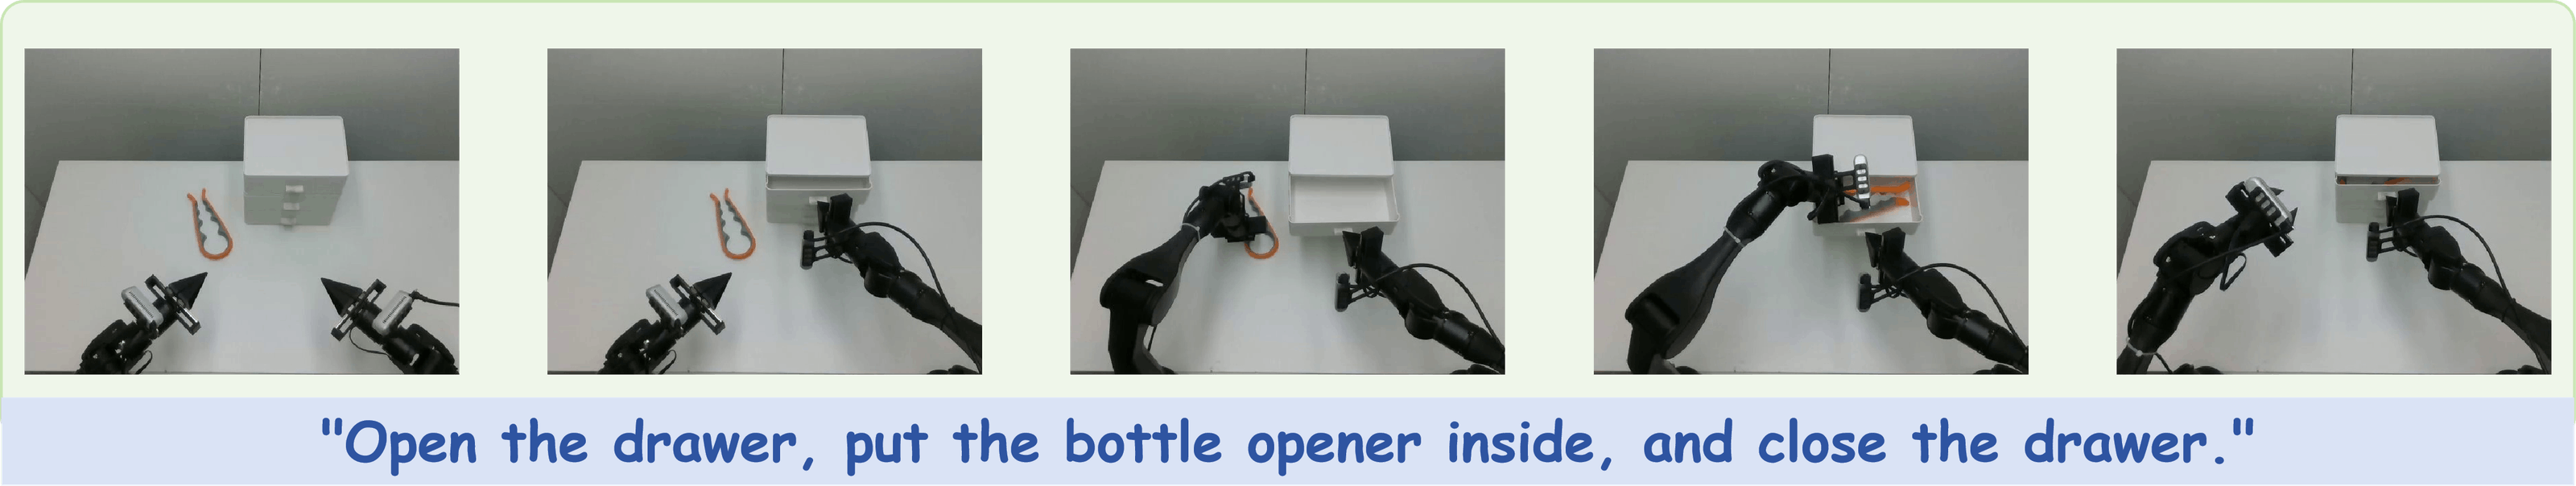
\includegraphics[width=0.95\linewidth]{figures/lyp/w1-04.png}

    \caption{
        Representative long-horizon tasks on the W1 robot platform.
        The examples demonstrate sequential manipulation behaviors in
        complex environments.
    }
    \label{fig:w1_tasks}
\end{figure}